The project has room for improvements and potential for new development directions. During the development, I used a git repository hosted on GitHub. I used the issues list from GitHub in order to have an overview of the problems that the application had. There are still a few issues opened and that I didn't have time to work with; some are bugs and others are ideas for future development. See \ref{fig:issues} to see an screenshot of this list.

\begin{figure}[h!]
    \setlength{\tempheight}{15ex}
    \centering
    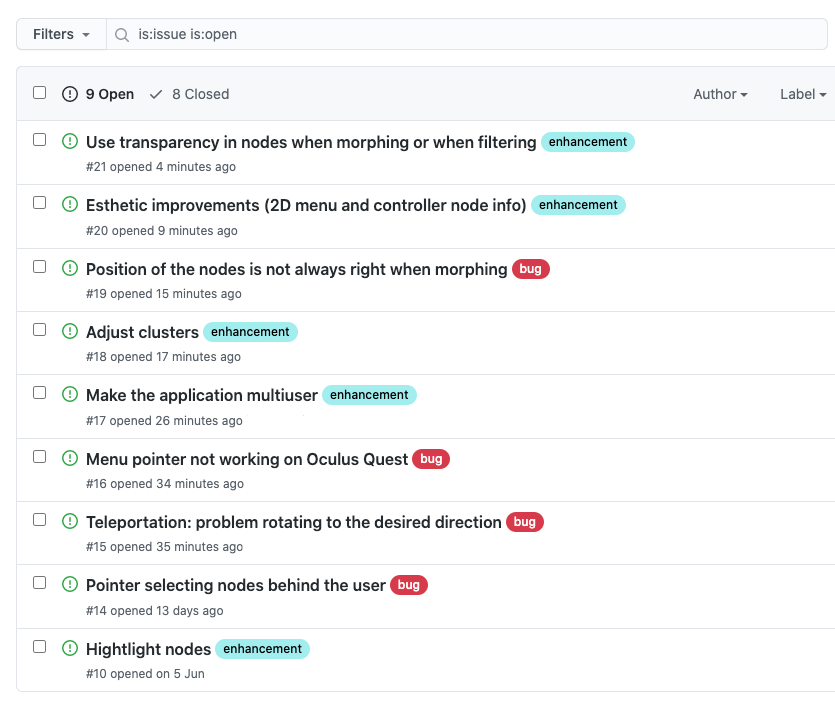
\includegraphics[width=\textwidth]{issues_github}
    \caption{List of issues from Github. They are tagged with "bug" or "enhancement" to specify what kind of issue it is about.}
    \label{fig:issues}
\end{figure}

As we can see in the list, there are some issues that are tagged as "bug"; These bugs are not very big and don't prevent the GeneNet VR from being functional. However, they impact upon the usability of the application.

A problem that we found out is that when the application is run on the Oculus Quest hardware, the pointer for the 2-dimensional menu dones't work. This can be a big problem since the user cannot use the filters or the morph slider. See issue with tag \#16. The other bugs are not so significant and can be read from the list. It's also possible to go to my GitHub account where a broader description for the issues can be found when clicking on them.

We believe that GeneNet VR has also potential for new development. In the list from GitHub, we wrote som ideas and we tagged them with the word "enhancement". Something that could be interesting is to make the application mulituser. We got this idea from CellexalVR\cite{cellexalvr}, where two people can be in the same session and only one of them can interact with the data, the other is only a watcher. We could implement something similar in GeneNet VR, where one of the users is just a watcher but can for instance teleport to other parts of the network to visualize it. This issue has the id \#17 in my list.

Another improvement that we think that would enhance the performance of the application, is to "prerender" the lines that correspond to the edges between the nodes during the initialization of the application and show them when they are needed. Right now, these lines are rendered in the scene every time a new node is selected. We use a function from Unity called Instantiate for this, which can downgrade the performance of the application, according to some forums from Unity.
It would be interesting to compare the performance using the Instantiate function with the solution that we propose to determine if Instantiate is a performance problem. The issue is referenced as \#22.

Other improvements for BigNet VR would be focused on teh aesthetics of the application. It's something that we haven't focused much since our main goal was that it was functional. An important issues is number \#21: now the nodes that we filter and that are morphed are turned into black colour. Instead it would be better to make the nodes transparent. If the nodes are still there but in black colour, they could hide other nodes that are behind them and the user might not see those nodes. Other ideas are for example hightlight the nodes that are selected and their related nodes (reference \#10), the possibility to adjust the clusters (reference \#18) and improve the 2D elements like the menu (\#20).

Finally, we would also like to run other experiments to further evaluate the application. For instance, we couldn't determine if the number of nodes had some impact in the scalability. It would be interesting to test the application with larger datasets and study the performance.

\section{Visualization of other abstract networks}
We developed GeneNet VR for the visualization of abstract networks with genetic data. We think that we could use GeneNet VR to visualize other networks of abstract data that have a similar structure: nodes and edges between the nodes. This could be apply for datasets from also medicine, sociology, social media networks, etc.
